\documentclass[11pt,a4paper]{ctexart}

\usepackage[margin=2.3cm]{geometry}
\usepackage{amsmath}
\usepackage{booktabs}
\usepackage{caption}
\usepackage{float}
\usepackage{graphicx}
\usepackage{hyperref}
\usepackage{xcolor}

\graphicspath{{../pic/}{../checkpoints/}{pic/}{checkpoints/}}
\emergencystretch=2em
\hypersetup{
  colorlinks=true,
  linkcolor=blue!60!black,
  urlcolor=blue!60!black,
  citecolor=blue!60!black
}

\newcommand{\studentName}{于翔}
\newcommand{\studentID}{23307130202}
\newcommand{\githubRepo}{\url{https://github.com/Parry-Git/Deep-Learning-Project2}}
\newcommand{\modelscopeRepo}{\url{https://www.modelscope.cn/models/ParryY/Deep-Learning-Project2}}
\newcommand{\bestPartOneAcc}{96.59\%}
\newcommand{\bestPartOneObservedAcc}{96.85\%}
\newcommand{\bestVggAcc}{90.52\%}

\title{\textbf{NNDL Project 2 Report}\\CIFAR-10 Classification and Batch Normalization}
\author{\studentName \quad \studentID}
\date{June 2026}

\begin{document}
\maketitle

\begin{abstract}
本项目围绕 CIFAR-10 图像分类完成两部分实验。第一部分设计并训练一个面向
32$\times$32 图像的残差卷积网络，系统比较网络宽度、激活函数、优化器、损失函数
和正则化强度对测试精度的影响。最终发布的 Part 1 checkpoint 采用中等宽度
CifarResNet，在 200 epoch 训练中取得 \bestPartOneAcc{} 的最佳测试精度；消融实验中
large-width 配置在 100 epoch 下达到 \bestPartOneObservedAcc{}，显示模型容量仍是主要
可提升方向。第二部分复现 VGG-A 与 VGG-A+BatchNorm 的对比，并通过多学习率训练轨迹
和 loss landscape band 解释 BN 对训练稳定性的贡献。100 epoch 对比中，VGG-A+BN 达到
\bestVggAcc{}，相比 VGG-A 的 87.61\% 提升 2.91 个百分点。
\end{abstract}

\section{Submission Links and Reproducibility}

\begin{table}[H]
\centering
\caption{Required submission links and released artifacts.}
\begin{tabular}{lp{0.66\linewidth}}
\toprule
Item & Link or Path \\
\midrule
Code repository & \githubRepo{} \\
Dataset and trained weights & \modelscopeRepo{} \\
Part 1 released checkpoint & \texttt{checkpoints/part1\_best.pth} \\
Part 2 released checkpoints &
\texttt{checkpoints/vgg\_bn/best\_vgg\_compare\_e100\_*.pth} \\
\bottomrule
\end{tabular}
\end{table}

\begin{table}[H]
\centering
\caption{Coverage of the project requirements.}
\begin{tabular}{p{0.24\linewidth}p{0.62\linewidth}}
\toprule
Requirement & Where it is addressed \\
\midrule
Identity and links &
Title page and Table 1. \\
Part 1 modules &
CifarResNet uses Conv2d, activation, global average pooling, fully connected layer, BatchNorm, Dropout, and residual shortcuts. \\
Part 1 ablations &
Table \ref{tab:part1-ablation} compares width/filter counts, activations, optimizers, losses, and regularization. \\
Visualization and insight &
Training curves, qualitative predictions, and ablation analysis in Section 2. \\
BN comparison &
VGG-A and VGG-A+BN training curves and accuracy table in Section 3.1. \\
Loss landscape &
Learning-rate sweep and loss landscape band analysis in Sections 3.2--3.3. \\
\bottomrule
\end{tabular}
\end{table}

所有实验均在同一份 CIFAR-10 数据集上完成，训练集 50,000 张、测试集 10,000 张。
代码仓库只保存源码、报告和复现实验脚本；数据集、训练日志、曲线图和模型权重不进入
Git，而是通过 ModelScope 发布。这样可以保持 GitHub 仓库轻量，同时保证评测者可以
通过如下命令下载数据与发布权重，并复现核心测试：

\begin{verbatim}
conda activate sii
pip install -r requirements.txt
python codes/download.py --all
python codes/part1_cifar10/test.py
\end{verbatim}

若需要从头复现实验，可进一步运行 Part 1 主训练、Part 1 消融脚本和 Part 2 批处理
脚本，具体命令见 GitHub README。核心依赖保持为 PyTorch、torchvision、matplotlib、
numpy 和 modelscope，避免引入不必要的环境复杂度。

\section{Part 1: CIFAR-10 Classifier}

\subsection{Architecture}

Part 1 使用自定义 CifarResNet，而不是直接调用 torchvision 中的现成分类器。网络包含
项目要求的 Conv2d、Pooling、Activation 和 Fully Connected 层，同时引入 BatchNorm、
Dropout 和 residual connection 作为稳定训练与提升泛化的组件。基础结构如下：

\[
\begin{aligned}
\mathrm{Conv}_{3\times3}(3 \rightarrow C_1)
&\rightarrow
\left[\mathrm{ResidualBlock}\right]^{3}_{C_1}
\rightarrow
\left[\mathrm{ResidualBlock}\right]^{3}_{C_2} \\
&\rightarrow
\left[\mathrm{ResidualBlock}\right]^{3}_{C_3}
\rightarrow
\mathrm{GAP}
\rightarrow
\mathrm{FC}_{10}.
\end{aligned}
\]

每个 residual block 含两个 $3\times3$ 卷积、两个 BatchNorm、一个可选 Dropout2d 和
shortcut 分支；阶段切换时通过 stride=2 下采样。最终采用 global average pooling
替代大规模全连接层，以减少参数量并提升平移鲁棒性。主模型配置为 channels
$(64,128,256)$、blocks $(3,3,3)$、ReLU、dropout 0.1，约 4.33M 参数。

\subsection{Training Setup}

训练数据增强包括 RandomCrop(32, padding=4)、RandomHorizontalFlip、标准 CIFAR-10
归一化和 Cutout(length=16)。优化器采用 SGD momentum 0.9，初始学习率 0.1，
weight decay $5\times10^{-4}$；学习率调度为 5 epoch warmup 后接 CosineAnnealing。
损失函数默认使用 label smoothing cross entropy，平滑系数为 0.1。训练默认开启 AMP，
在 CUDA 上使用 float16 autocast 和 GradScaler；它主要降低训练时间和显存占用，未改变
模型结构或评价流程。

\begin{table}[H]
\centering
\caption{Part 1 main run configuration and result.}
\begin{tabular}{ll}
\toprule
Item & Value \\
\midrule
Model & CifarResNet, blocks $(3,3,3)$, channels $(64,128,256)$ \\
Optimizer & SGD, momentum 0.9, weight decay $5\times10^{-4}$ \\
Loss & Cross entropy with label smoothing 0.1 \\
Scheduler & 5-epoch warmup + cosine annealing \\
Epochs / batch size & 200 / 128 \\
Best test accuracy & \bestPartOneAcc{} at epoch 195 \\
Final test accuracy & 96.52\% \\
\bottomrule
\end{tabular}
\end{table}

\begin{figure}[H]
\centering
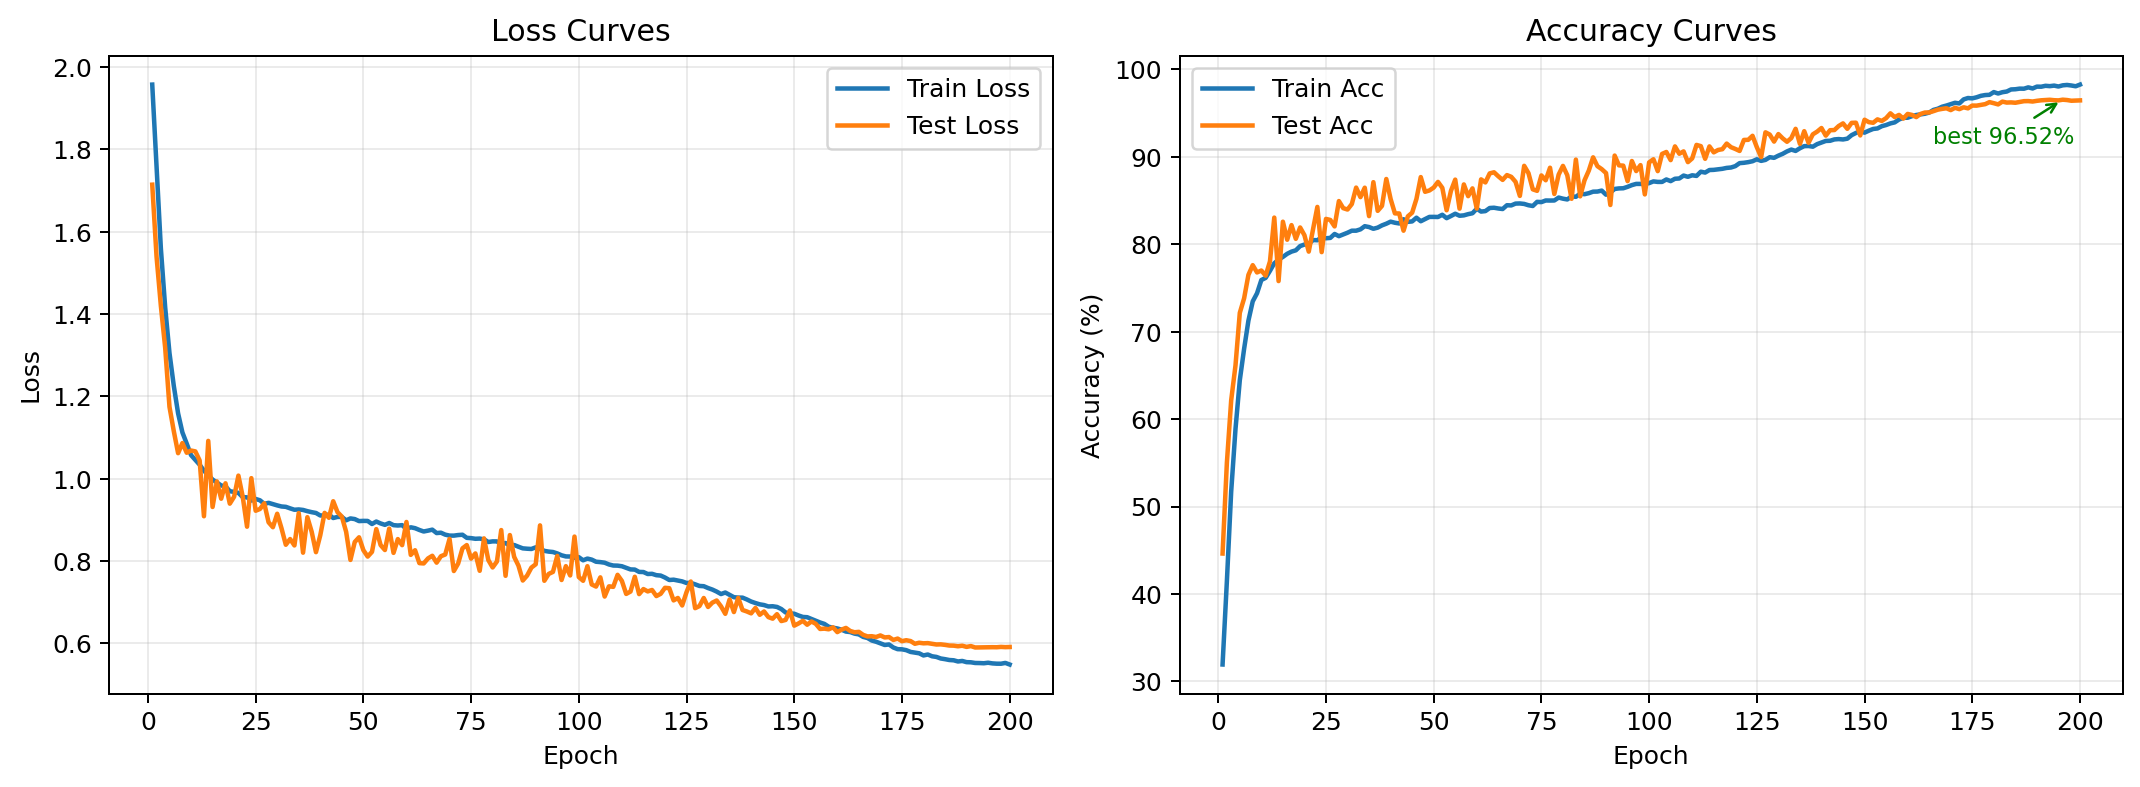
\includegraphics[width=\linewidth]{training_curves_main_sgd.png}
\caption{Training and test curves of the released Part 1 model.}
\end{figure}

\subsection{Ablation Study}

为避免单个超参数结论被其它因素混淆，消融实验均以相同的数据增强、batch size、
100 epoch、cosine schedule 和默认 AMP 为基础，只改变一组变量。表
\ref{tab:part1-ablation} 汇总了所有 Part 1 消融实验。

\begin{table}[H]
\centering
\scriptsize
\caption{Part 1 ablation results on CIFAR-10.}
\label{tab:part1-ablation}
\begin{tabular}{llllrr}
\toprule
Group & Variant & Main changed setting & Optimizer/Loss & Best Acc. & Final Acc. \\
\midrule
Width & Small & channels $(32,64,128)$ & SGD / LS 0.1 & 94.67 & 94.48 \\
Width & Medium & channels $(64,128,256)$ & SGD / LS 0.1 & 96.30 & 96.29 \\
Width & Large & channels $(128,256,512)$ & SGD / LS 0.1 & \textbf{96.85} & 96.77 \\
\midrule
Activation & ReLU & activation=ReLU & SGD / LS 0.1 & \textbf{96.28} & 96.24 \\
Activation & GELU & activation=GELU & SGD / LS 0.1 & 95.71 & 95.62 \\
Activation & SiLU & activation=SiLU & SGD / LS 0.1 & 95.12 & 95.09 \\
\midrule
Optimizer & SGD & lr=0.1 & LS 0.1 & \textbf{96.15} & 96.09 \\
Optimizer & Adam & lr=0.001 & LS 0.1 & 95.23 & 95.06 \\
Optimizer & AdamW & lr=0.001 & LS 0.1 & 95.26 & 95.21 \\
\midrule
Loss & CE & label smoothing=0 & SGD & 96.10 & 96.03 \\
Loss & LS 0.05 & label smoothing=0.05 & SGD & \textbf{96.39} & 96.35 \\
Loss & LS 0.10 & label smoothing=0.10 & SGD & 96.33 & 96.33 \\
Loss & Focal & $\gamma=2.0$ & SGD & 95.52 & 95.46 \\
\midrule
Reg. & Dropout 0.0 & dropout=0.0 & SGD / LS 0.1 & \textbf{96.28} & 96.22 \\
Reg. & Dropout 0.1 & dropout=0.1 & SGD / LS 0.1 & 96.12 & 96.07 \\
Reg. & Dropout 0.2 & dropout=0.2 & SGD / LS 0.1 & 95.83 & 95.76 \\
Reg. & WD $10^{-4}$ & weight decay=$10^{-4}$ & SGD / LS 0.1 & 95.80 & 95.69 \\
\bottomrule
\end{tabular}
\end{table}

主要结论如下。第一，网络宽度是最明显的性能因素：从 small 到 medium 提升 1.63 个
百分点，从 medium 到 large 进一步提升 0.55 个百分点。这说明当前误差仍有一部分来自
模型容量限制，但 large-width 的计算和存储成本也显著增加，因此发布权重选择了更均衡
的 medium-width 200 epoch 模型。第二，在本网络和训练设置下，ReLU 优于 GELU 和 SiLU。
这并不说明 ReLU 总是更好，而是说明当前残差块、BatchNorm 和 Kaiming 初始化与 ReLU
匹配更直接，训练到 100 epoch 时泛化更稳定。第三，SGD+momentum 明显优于 Adam/AdamW；
Adam 系列前期收敛快，但最终测试精度低约 0.9 个百分点，符合图像分类中 SGD 往往具有
更好泛化的经验。第四，适度 label smoothing 有帮助，其中 0.05 略优于 0.10；focal loss
在类别均衡的 CIFAR-10 上没有优势。第五，Dropout 并非越大越好。当前模型已有数据增强、
weight decay、BatchNorm 和残差结构，dropout 0.2 会产生欠拟合倾向。

\begin{figure}[H]
\centering
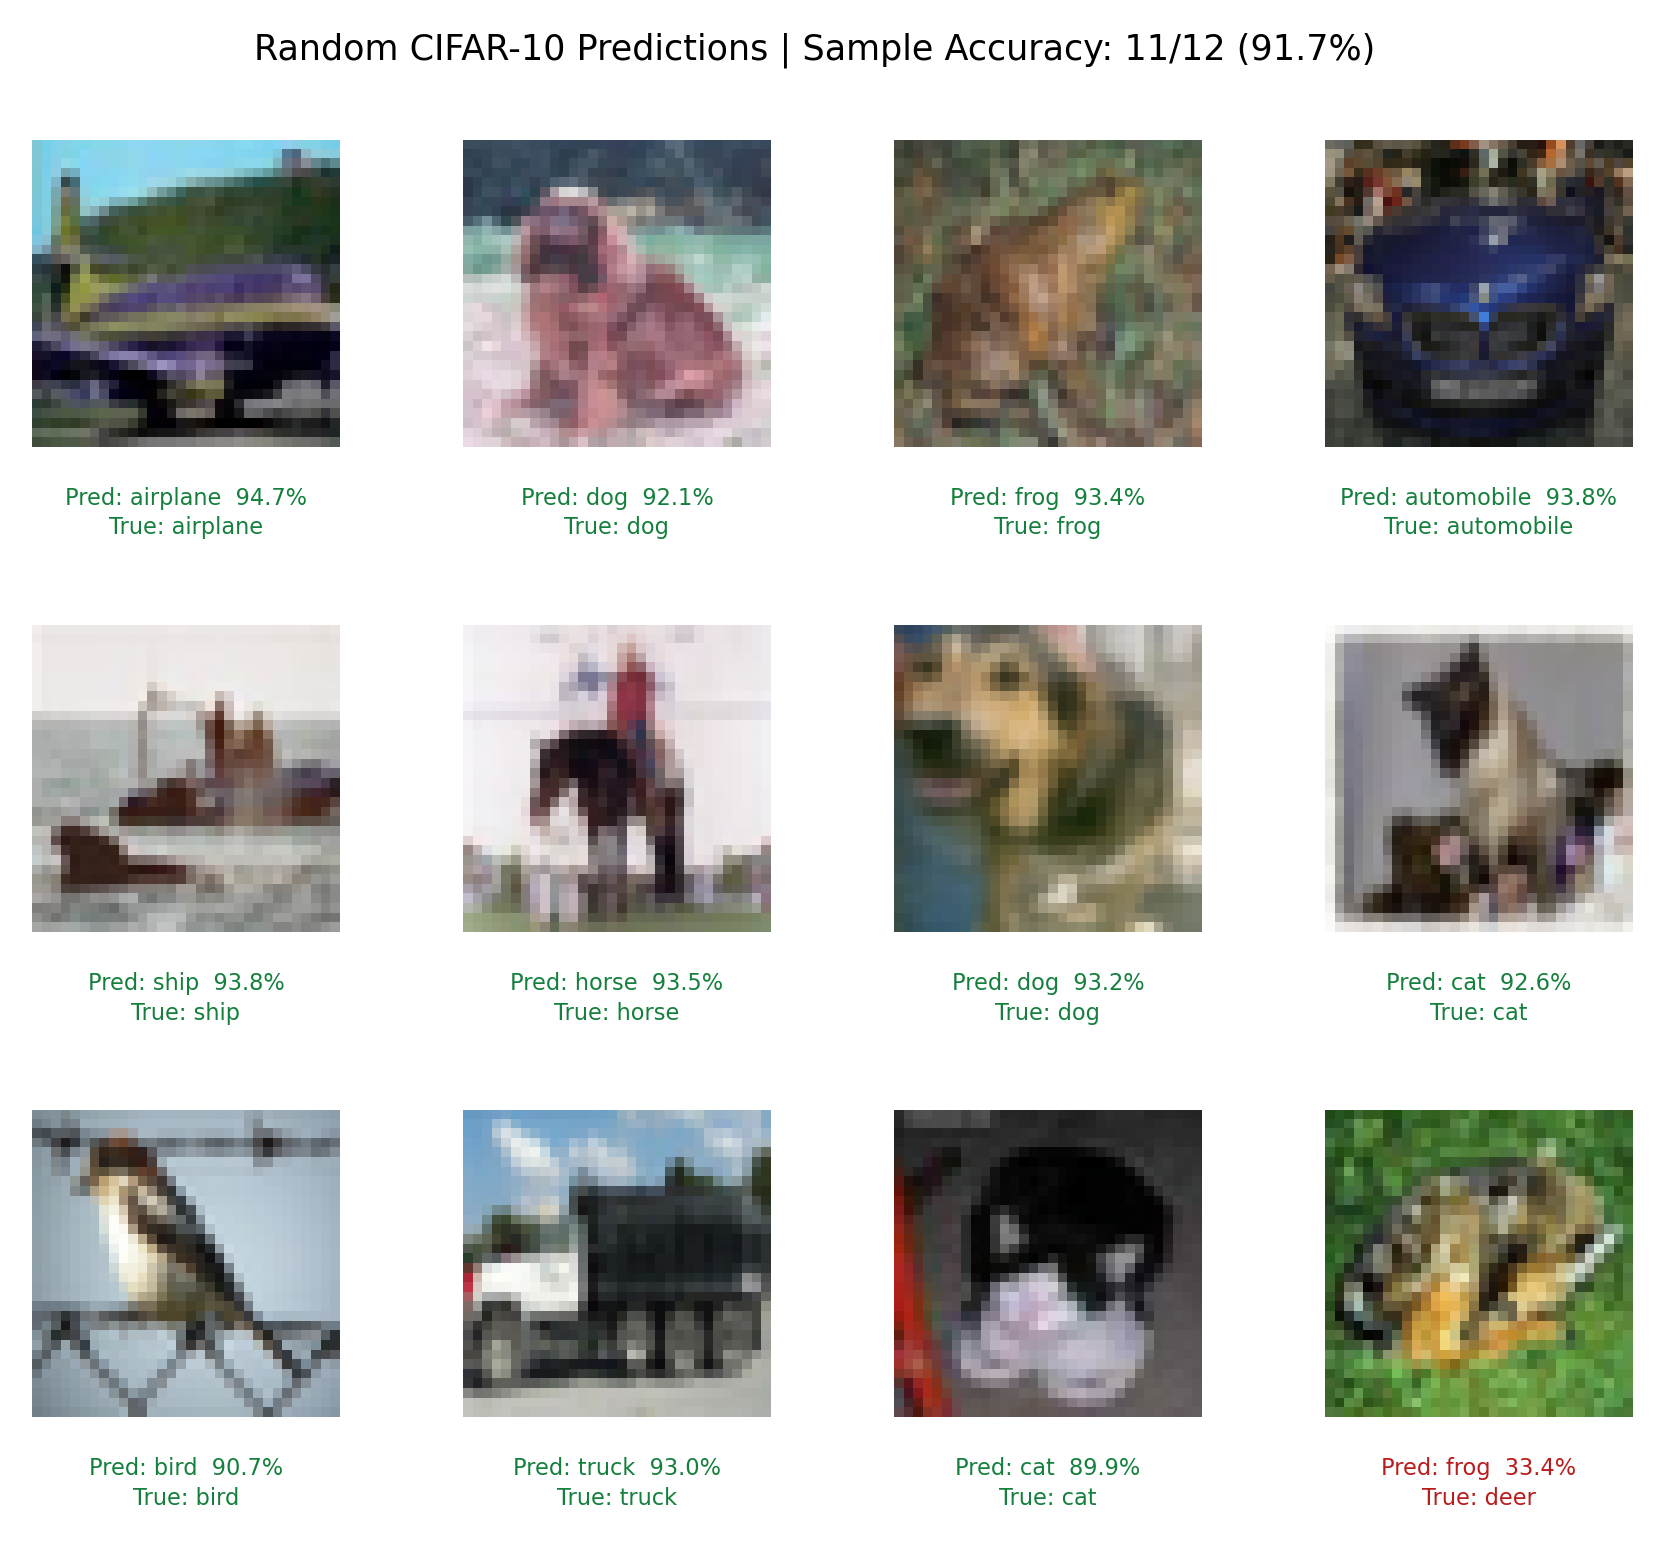
\includegraphics[width=0.78\linewidth]{predictions.png}
\caption{Qualitative predictions from the released Part 1 checkpoint.}
\end{figure}

\section{Part 2: Batch Normalization}

\subsection{VGG-A and VGG-A+BN Setup}

Part 2 使用 VGG-A 作为 baseline，并在每个卷积层之后加入 BatchNorm2d 构成
VGG-A+BN。两者除 BN 之外保持一致：5 个卷积 stage、MaxPool 下采样、三层 classifier，
输入分辨率仍为 CIFAR-10 的 32$\times$32。VGG-A 有 9,750,922 个参数，VGG-A+BN 有
9,753,674 个参数；参数量差异很小，因此性能差异主要来自 BN 的优化效果，而不是容量。

\begin{table}[H]
\centering
\caption{VGG-A vs VGG-A+BN, 100 epochs, Adam lr=$10^{-3}$.}
\begin{tabular}{lrrrr}
\toprule
Model & Params & Best Acc. & Best Epoch & Final Acc. \\
\midrule
VGG-A & 9,750,922 & 87.61 & 99 & 86.58 \\
VGG-A+BN & 9,753,674 & \textbf{90.52} & 98 & 90.30 \\
\bottomrule
\end{tabular}
\end{table}

\begin{figure}[H]
\centering
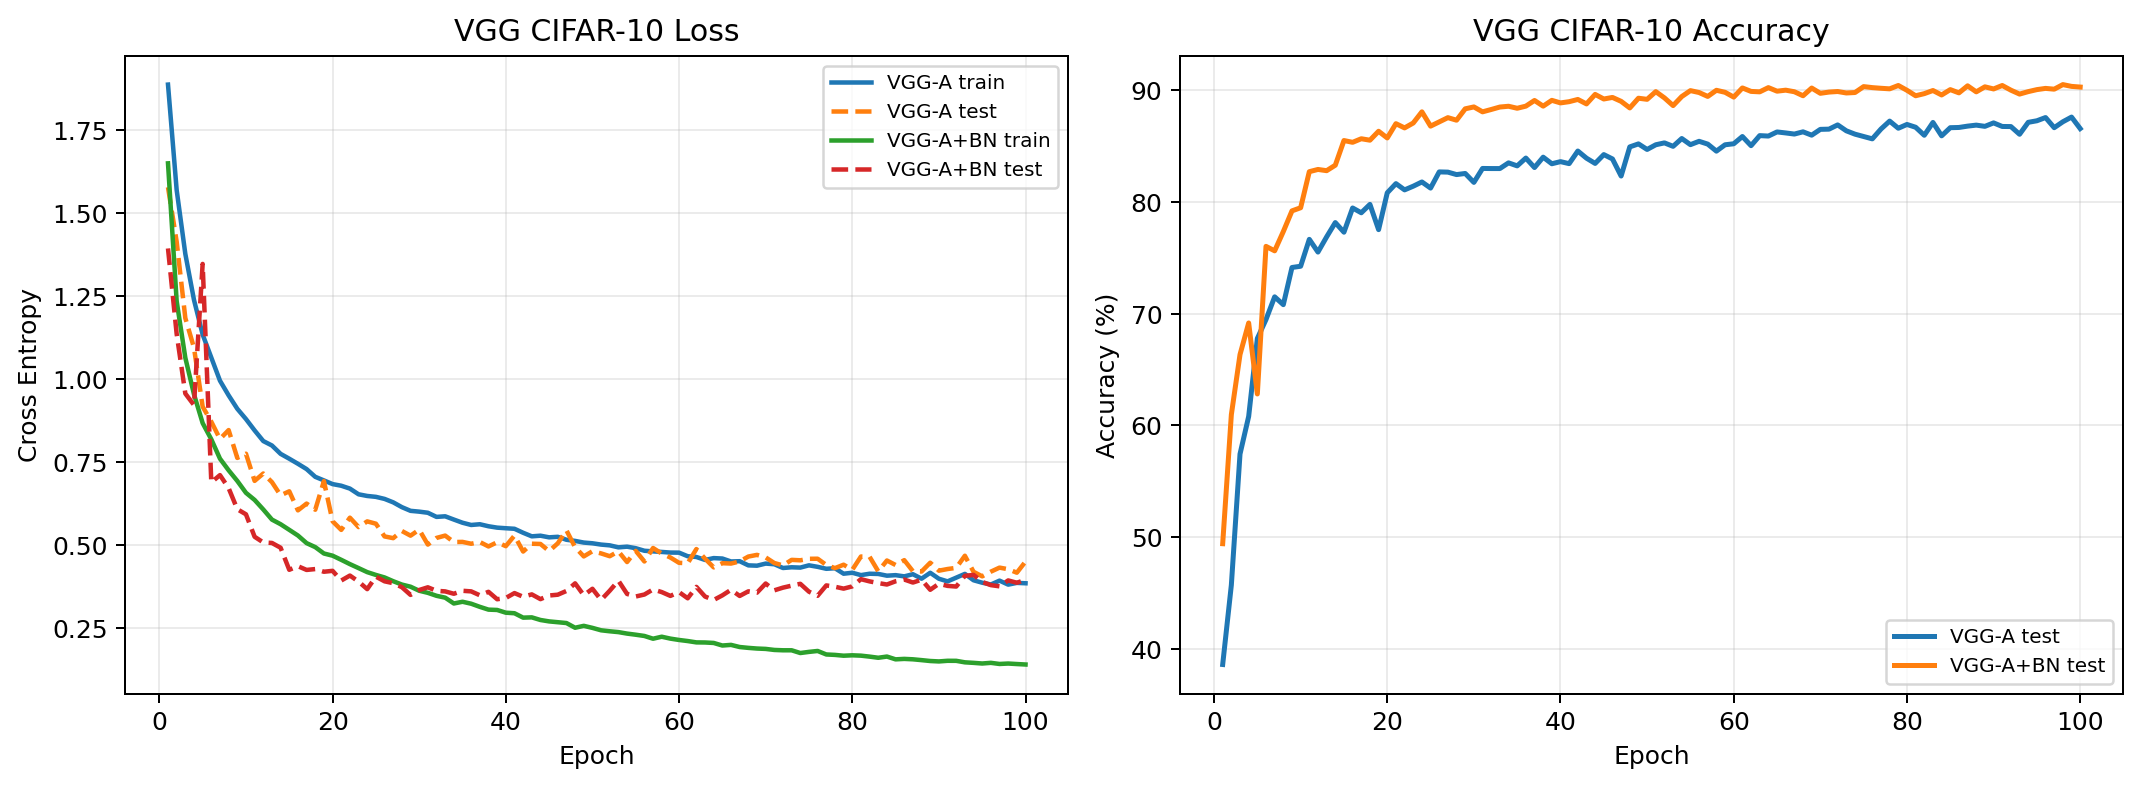
\includegraphics[width=\linewidth]{vgg_train_vgg_compare_e100.png}
\caption{Training curves for VGG-A and VGG-A+BN. BN improves both convergence and final accuracy.}
\end{figure}

从曲线可以看出，VGG-A+BN 在训练早期更快进入有效下降区间，测试精度曲线也更加平滑。
在 100 epoch 结束时，BN 版本 final accuracy 为 90.30\%，而无 BN 的 VGG-A 为
86.58\%。这说明 BN 不只是提高最终精度，也改善了训练过程的可控性。

\subsection{Learning Rate Sensitivity}

为了进一步检查 BN 的稳定性，实验在 $\{10^{-4}, 5\times10^{-4}, 10^{-3}, 2\times10^{-3}\}$
四个学习率下分别训练 40 epoch。结果如表 \ref{tab:vgg-lr} 所示。

\begin{table}[H]
\centering
\caption{Learning-rate sweep for VGG-A and VGG-A+BN.}
\label{tab:vgg-lr}
\begin{tabular}{lrrrr}
\toprule
Learning rate & VGG-A Best & VGG-A Final & VGG-A+BN Best & VGG-A+BN Final \\
\midrule
$1\times10^{-4}$ & 85.14 & 84.30 & 86.24 & 85.97 \\
$5\times10^{-4}$ & 86.51 & 86.39 & 89.54 & 89.54 \\
$1\times10^{-3}$ & 83.68 & 83.44 & 89.46 & 89.46 \\
$2\times10^{-3}$ & 76.64 & 75.45 & 89.38 & 89.02 \\
\bottomrule
\end{tabular}
\end{table}

无 BN 的 VGG-A 对学习率非常敏感：当 lr 从 $5\times10^{-4}$ 增加到 $2\times10^{-3}$
时，best accuracy 从 86.51\% 降到 76.64\%。相反，VGG-A+BN 在后三个学习率下都稳定在
约 89.4\% 左右。这支持了 BN 能扩大可用学习率区间、降低调参敏感性的结论。

\begin{figure}[H]
\centering
\begin{minipage}{0.49\linewidth}
\centering
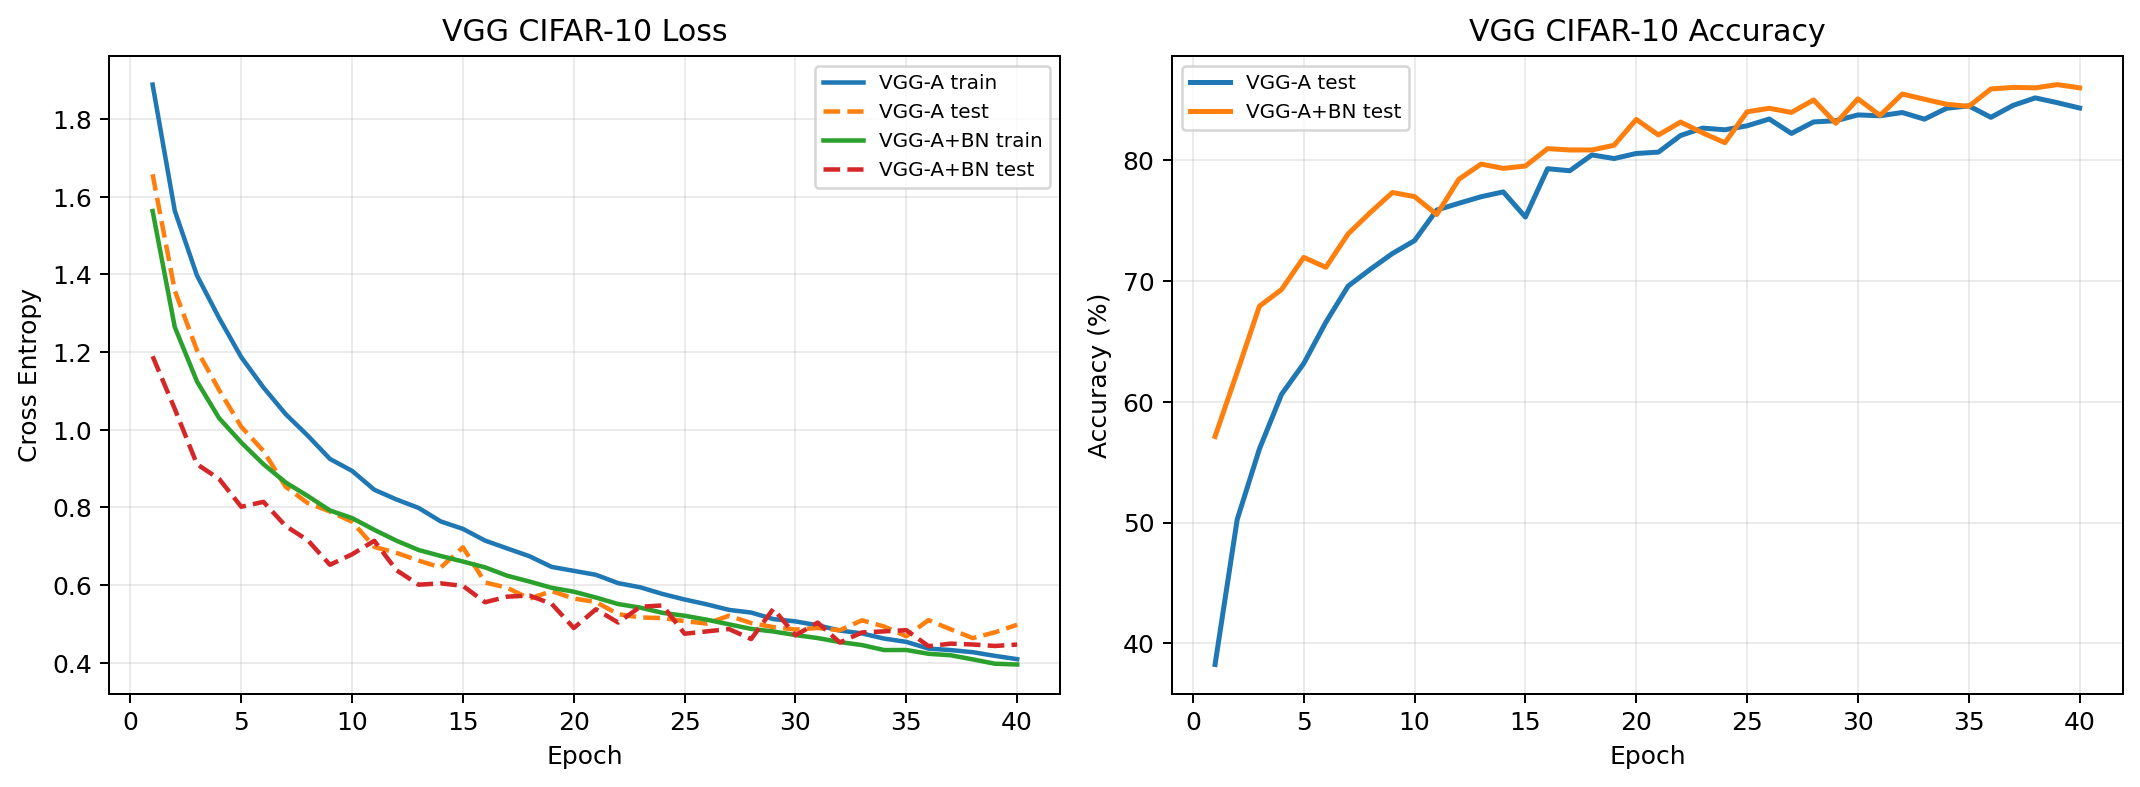
\includegraphics[width=\linewidth]{vgg_train_vgg_lr_0p0001_e40.png}
\caption*{lr=$10^{-4}$}
\end{minipage}
\begin{minipage}{0.49\linewidth}
\centering
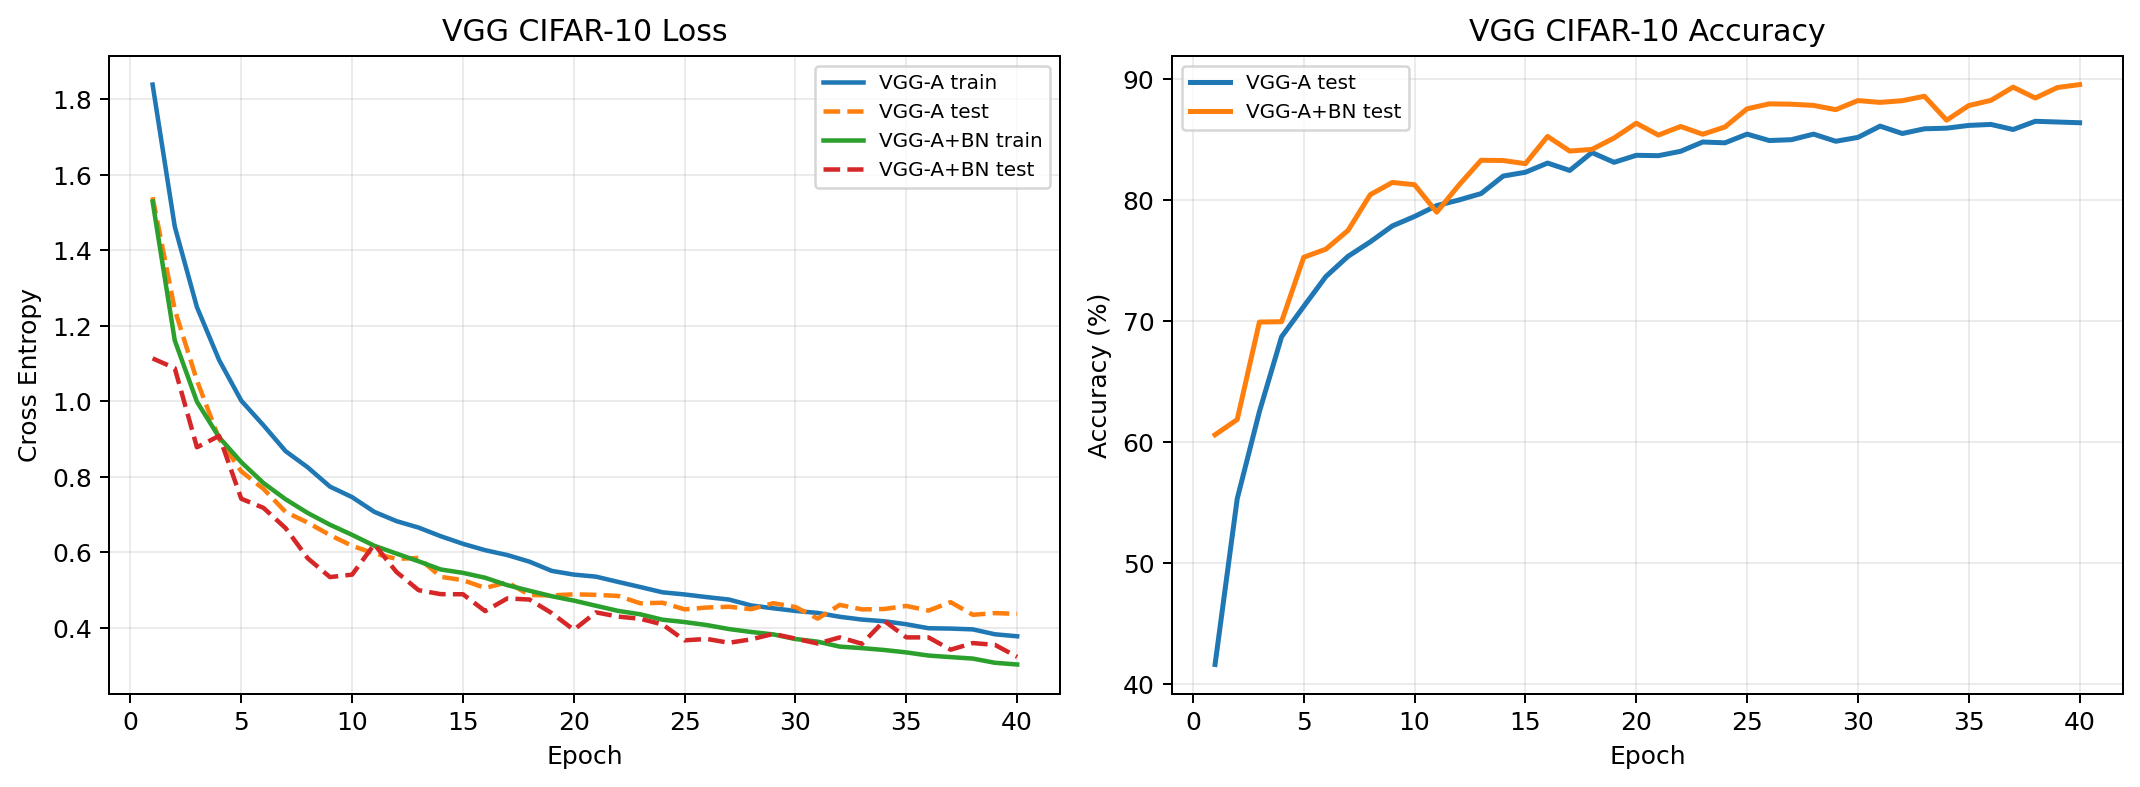
\includegraphics[width=\linewidth]{vgg_train_vgg_lr_0p0005_e40.png}
\caption*{lr=$5\times10^{-4}$}
\end{minipage}
\begin{minipage}{0.49\linewidth}
\centering
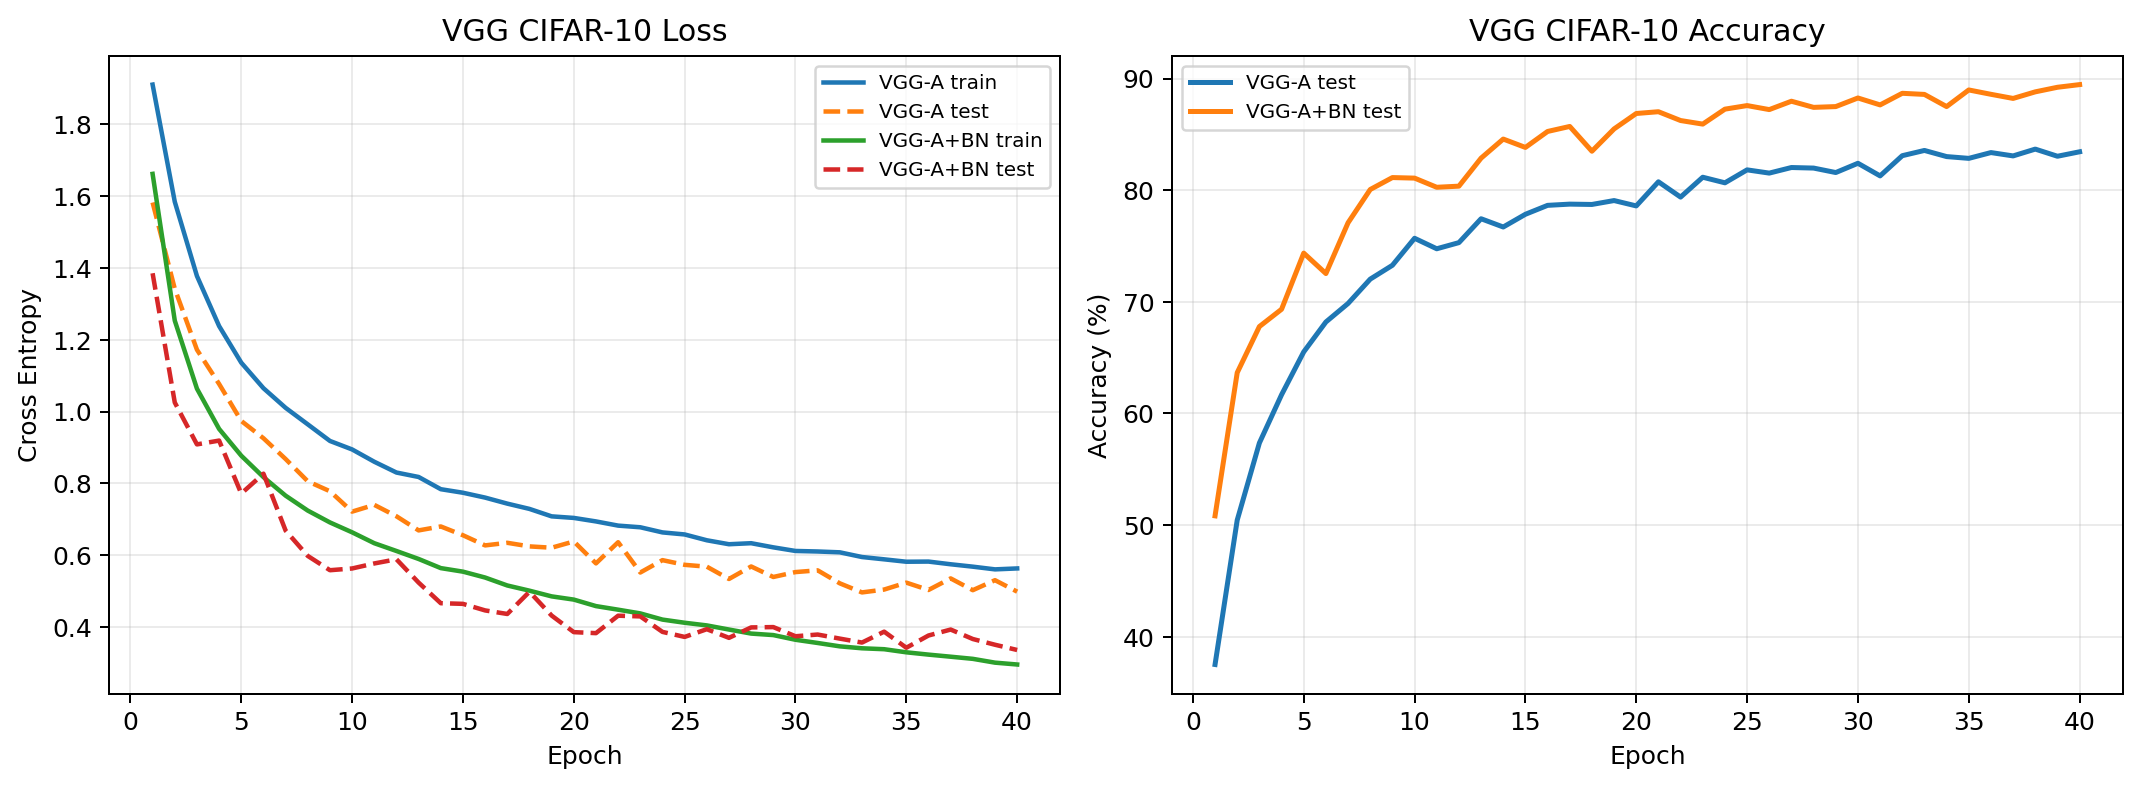
\includegraphics[width=\linewidth]{vgg_train_vgg_lr_0p001_e40.png}
\caption*{lr=$10^{-3}$}
\end{minipage}
\begin{minipage}{0.49\linewidth}
\centering
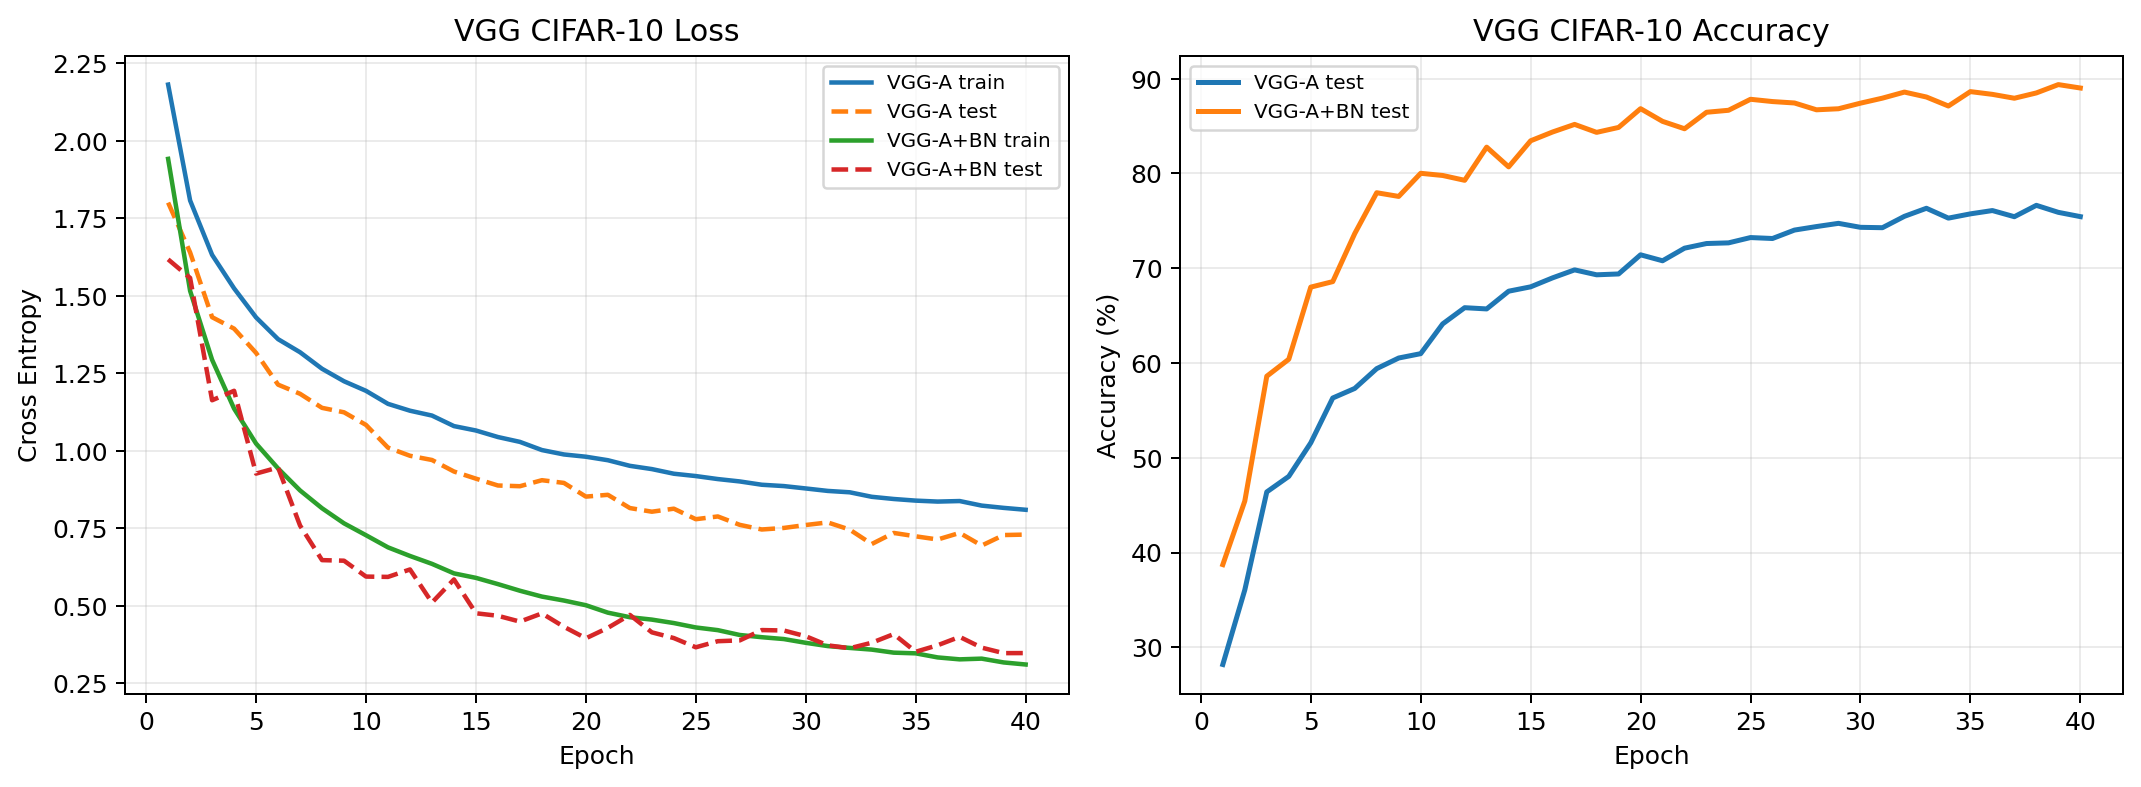
\includegraphics[width=\linewidth]{vgg_train_vgg_lr_0p002_e40.png}
\caption*{lr=$2\times10^{-3}$}
\end{minipage}
\caption{VGG learning-rate sweep curves. BN keeps the curves stable under larger learning rates.}
\end{figure}

\subsection{Loss Landscape}

Loss landscape 实验记录四个学习率下每个模型的 mini-batch loss，并对同一步的多条
loss 曲线取上下界，形成 ``band''。band 越宽，说明同一训练阶段对学习率越敏感；
最终平均 loss 越低，说明对应设置更容易到达有效优化区域。

\begin{table}[H]
\centering
\caption{Loss landscape band statistics.}
\begin{tabular}{lrrr}
\toprule
Model & Mean Band Width & Max Band Width & Final Mean Loss \\
\midrule
VGG-A & 0.7475 & 18.0730 & 2.0057 \\
VGG-A+BN & 1.3808 & 5.7247 & \textbf{1.3629} \\
\bottomrule
\end{tabular}
\end{table}

\begin{figure}[H]
\centering
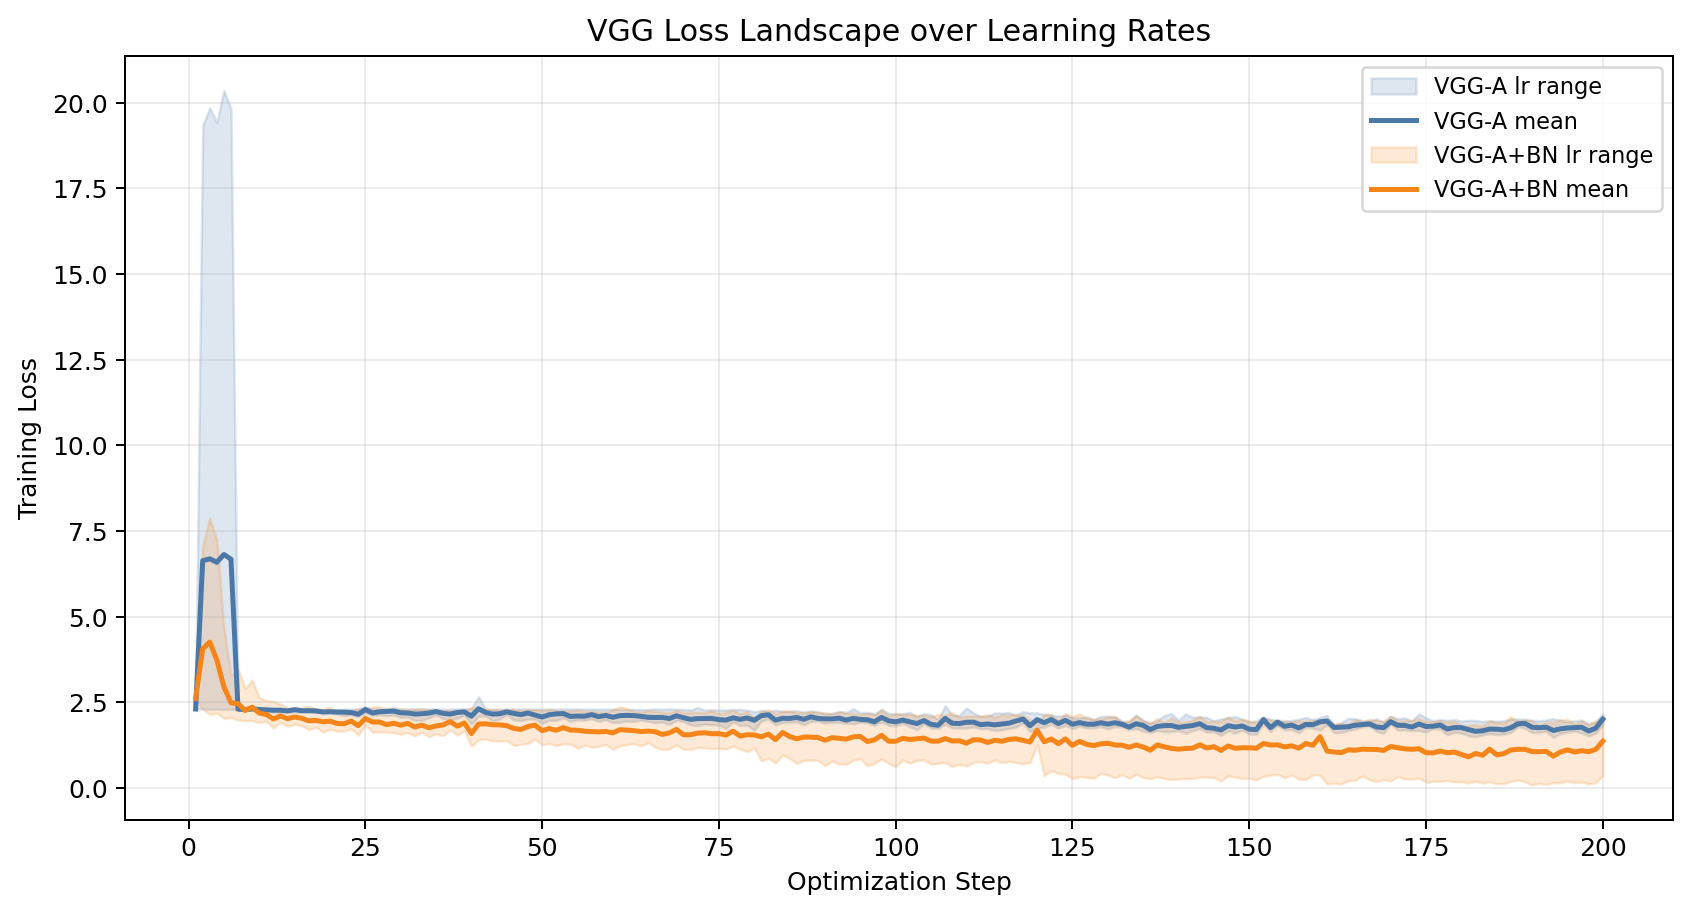
\includegraphics[width=0.90\linewidth]{loss_landscape_vgg_loss_landscape.png}
\caption{Loss landscape bands across learning rates. BN substantially lowers final mean loss and avoids the extreme loss spike observed without BN.}
\end{figure}

虽然 BN 的平均 band width 更大，但其最大 band width 只有 VGG-A 的约三分之一，且最终
平均 loss 明显更低。结合学习率 sweep 可知，无 BN 模型在部分学习率下会出现剧烈损失
峰值并最终停在较差区域；BN 通过规范化中间激活，缓解了层间尺度漂移，使梯度更新在
更宽的学习率范围内保持有效。

\section{Discussion}

Part 1 的结果表明，在 CIFAR-10 这类小尺寸图像任务上，一个专门设计的残差 CNN 可以
在不依赖预训练模型的情况下达到 96\% 以上测试精度。最有效的因素是足够的卷积宽度、
SGD + momentum、cosine schedule 和适度 label smoothing。相较之下，更复杂的激活函数和
focal loss 没有带来收益，说明模型改进需要结合数据分布和优化设置，而不是简单堆叠
技巧。

Part 2 的结果清楚显示 BN 的价值主要体现在优化稳定性上。VGG-A 与 VGG-A+BN 参数量
几乎相同，但 BN 版本在主实验中高 2.91 个百分点，在高学习率设置下优势扩大到十几个
百分点。loss landscape 进一步说明，BN 减少了极端 loss spike，并使模型更容易到达
低损失区域。

当前仍有两个可改进点。第一，large-width Part 1 消融达到 96.85\%，超过发布的
medium-width checkpoint；如果最终目标是单纯追求最高准确率，可以额外训练并发布
large-width 200 epoch 权重。第二，当前 Part 2 的目标是分析 BN 的优化作用，而不是
超过 Part 1 的专用残差分类器；因此 VGG-A+BN 精度低于 CifarResNet 是符合预期的。

\section{Conclusion}

本项目完成了 CIFAR-10 自定义 CNN 训练、系统消融实验、VGG-A BatchNorm 对比实验以及
loss landscape 分析。Part 1 发布模型达到 \bestPartOneAcc{}，消融实验最高观察精度为
\bestPartOneObservedAcc{}；Part 2 中 VGG-A+BN 达到 \bestVggAcc{}，明显优于无 BN
baseline。整体实验结果相互支撑：残差结构、合适正则化和稳健优化策略决定最终分类
性能，而 BatchNorm 的核心作用是改善优化条件、扩大稳定学习率范围并降低训练失败风险。

\end{document}
